% Predlozak za pisanje diplomskog rada na PMF-MO
% Opcenita uputstva za LaTeX se mogu npr. naci na 
% http://web.math.hr/nastava/rp3, http://web.math.hr/nastava/s4-prof/latex.pdf

\documentclass[a4paper,oneside,12pt]{memoir} % jednostrano: promijeniti twoside u oneside
% Paket inputenc omogucava direktno unosenje hrvatskih dijakritickih znakova 
% opcija utf8 za unicode (unix, linux, mac)
% opcija cp1250 za windowse
\usepackage[utf8]{inputenc}  % ukoliko se koristi XeLaTeX onda je \usepackage{xunicode}\usepackage{xltxtra}
% Stil za diplomski, unutra je ukljucena podrska za hrvatski jezik
\usepackage{diplomski}
% bibliografija na hrvatskom
\usepackage[languagenames,fixlanguage,croatian]{babelbib} % zahtijeva datoteku croatian.bdf
\usepackage{indentfirst}

% hiperlinkovi 
\usepackage[pdftex]{hyperref} % ukoliko se koristi XeLaTeX onda je \usepackage[xetex]{hyperref}
% Odabir familije fontova:
% koristenjem XeLaTeX-a mogu se koristiti svi fontovi instalirani na racunalu, npr
% \defaultfontfeatures{Mapping=tex-text}
% \setmainfont[Ligatures={Common}]{Hoefler Text}
% ili
% \newcommand{\nas}[1]{\fontspec{Adobe Garamond Pro}\fontsize{24pt}{24pt}\color{Chocolate}\selectfont #1}
% i onda \nas{Naslov ...}
\usepackage{txfonts} % times new roman 
% Paket graphicx sluzi za manipuliranje grafikom 
\usepackage[pdftex]{graphicx} % ukoliko se koristi XeLaTeX onda je \usepackage[xetex]{graphicx}
% Paket amsmath je vec ukljucen
% Dodatno definirane matematicke okoline:
% teorem (okolina: thm), lema (okolina: lem), korolar (okolina: cor),
% propozicija (okolina: prop), definicija (okolina: defn), napomena (okolina: rem),
% slutnja (okolina: conj), primjer (okolina: exa), dokaz (okolina: proof)
% Definirane su naredbe za ispisivanje skupova N, Z, Q, R i C
% Definirane su naredbe za funkcije koje se u hrvatskoj notaciji oznacavaju drukcije 
% nego u americkoj: tg, ctg, ... (\tgh za tangens hiperbolni)
% Takodjer su definirane naredbe za Ker i Im (da bi se razlikovala od naredbe za imaginarni dio kompleksnog broja, naredba se zove \slika).
\usepackage{algorithm2e} % http://ctan.org/pkg/algorithm2e
\usepackage[numbered, framed]{mcode}
\usepackage{indentfirst}
\usepackage{enumitem}
\usepackage{chngcntr}

\renewcommand\thechapter{\arabic{chapter}.}
\renewcommand\thesection{\arabic{chapter}.\arabic{section}.}
\renewcommand{\thethm}{\arabic{chapter}.\arabic{section}.\arabic{thm}}
\renewcommand{\thefigure}{\arabic{chapter}.\arabic{figure}.}
\usepackage[labelsep=space]{caption}
\captionsetup[figure]{labelfont=bf}
\renewcommand{\chaptermark}[1]{\markright{\uppercase{\thechapter~~#1}}}
\renewcommand{\lstlistingname}{Programski kod}

% Podaci o diplomskom radu
\title{Sustavi za davanje preporuka}
\author{Zlatko Damijanić}
\advisor{izv. prof. dr. sc. Luka Grubišić}  % obavezno s titulom
\date{rujan, 2017.}  % oblika mjesec, godina
\dedication{Obitelj, prijatelji, škola, izreka} % posveta

\begin{document}
\renewcommand\thelstlisting{\arabic{chapter}.\arabic{lstlisting}.}
\bibliography{ieetr}

\frontmatter % generira stranicu za potpise povjerenstva, posvetu i sadržaj
% uvod
\begin{intro}
Web, kažu, izlazi iz doba pretrage i ulazi u doba preporuka. Koja je razlika? Pretraga je kada tražimo nešto, a preporuka je kada nešto dobro za što nisi znao da postoji ili nisi znao kako pronaći, pronađe tebe. Informacijsko doba uslijedilo je nakon industrijskog doba i obilježeno je naglim razvitkom i raspostranjenosti informacijske tehnologije pomoću kojih informacije postaju sve dostupnije. Internet i digitalna tehnologija pružaju nove prilike za učenje, omogućuju pojedincima direktnu prodaju ideja, usluga ili proizvoda, pristup informacijama te zadovoljavanje emocionalnih i psiholoških potreba. Povećanjem količine informacije koja nas okružuje javlja se potreba za što boljim upravljanjem informacijama. Bitan aspekt tog upravljanja je filtriranje informacija koja se postiže pretragom ili preporukom. Kod pretrage korisnik upisuje ključne riječi te se na temelju unesenih riječi filtriraju informacije i prikazuju korisniku. Najpoznatiji primjer filtriranja je web tražilica Google koja pretražuje web stranice. Dok preporuke otkrivaju sadržaj na Internetu koji bi mogao biti zanimljiv korisniku na temelju nekih njegovih prethodno pregledanih sadržaja te zatim na temelju tih predviđanja dati mu listu od nekoliko preporuka. Filtriranje se može izvesti i njihovom kombinacijom. Među najpoznatijim primjerima sustava za  preporuku na webu su oni od tvrtke Amazon i Netflix.
% odlomak
\par 
U ovom radu opisan je općeniti sustav za davanje preporuka na webu i njegove zadaće. Dana je njihova podjela i opisani su algoritmi najkorištenijih predstavnika pojedine kategorije. Navedeni su njihovi nedostaci i prednosti te kako ih se može evaluirati.
\end{intro}
% poglavlje
\chapter{Opis i podjela sustava za davanje preporuka na webu}	
Sustav za davanje preporuka (eng. recommendation systems) spada u područje filtriranje informacija i čini ga skup metoda s kojima analizira dostupne podatke kako bi predvidio što bi se moglo svidjeti, što bi moglo zanimati ili što je relevantno za korisnika. Najčešći oblik preporuka je lista sadržaja za koje je sustav predvidio da su najrelevantniji za korisnika. Primarni razlog potrebe za takvim sustavima je previše raspoloživih informacija (eng. information overload) i raznih mogćnosti interakcije (eng. interaction overload), na primjer: pregledavanje, kupovanje, označavanje, ocjenjivanje, komentiranje, praćenje itd. Web mjesta kako bi korisnicima olakšali pronalaženje i dostupnost informacija te time povećali posjećnost i profitabilnost implementiraju sustave za davanje preporuka. Područje primjene sustava je veliko što se može vidjeti i iz sljedećih primjera.
% lista
\bigskip
\\ Primjeri web mjesta koje daju preporuke svojim korisnicima i područje njihove primjene:
\begin{itemize}[topsep=2pt]
\setlength{\parskip}{0pt}
\item movielens.org, netflix.com, imdb.com, themoviedb.org - filmovi
\item last.fm, pandora.com, spotify.com, napster.com - glazba
\item flickr.com, instagram.com, pinterest.com, imgur.com - slike
\item amazon.com, ebay.com, aliexpress.com, alibaba.com - e-trgovina
\item youtube.com, dailymotion.com, vimeo.com, metacafe.com - video
\item del.icio.us, diigo.com, raindrop.io, getpocket.com - web oznake 
\item facebook.com, myspace.com, linkedin.com, gotinder.com - prijatelji
\item airbnb.com, booking.com, trivago.com, tripping.com - smještaj
\item bibsonomy.org, citeulike.org, mendeley.com, zotero.org - publikacije
\item google.com/adsense, propellerads.com, media.net, infolinks.com - oglasi
\end{itemize}
\bigskip
% odlomak
\par
Problem preporuka definiran je 90-tih godina, ali se danas još razvija i poširuje se područje njegove primjene. 2006. godine problem je populariziran natjecanjem "Netflix Prize". Netflix je web mjesto za gledanje filmova, serija, emisija, TV kanala i sl. Natjecanje je bilo otvorenog tipa i cilj je bio pronaći algoritam koji će poboljšati predikcije Netflix-ovog algoritma. Trebalo je predvidjeti koju će ocjenu korisnik dodijeliti nekom filmu samo na temelju prijašnjih ocjena korisnika, bez dodatnih informacija o korisnicima i filmovima. Nagradu od 1.000.000 američkih dolara odnio je tim "BellKor's Pragmatic Chaos" koji je poboljšao predikcije za 10.06\%.
% odlomak
\par
Sustave za davanje preporuka dijelimo na nepersonalizirane i personalizirane. Nepersonalizirani sustavi su najednostavniji i ne uzimaju u obzir preferencije korisnike te daju svim korisnicima jednake preporuke. Prednost je što su jednostavni za implementaciju i lako je prikupiti podatke. Zbog širokog spektra područja primjene izraz sadržaj odnosi se na knjige, filmovi, video, proizvodi i ostalo što sustav preporučuje.   
% slika
\begin{figure}[!h]
\begin{center}
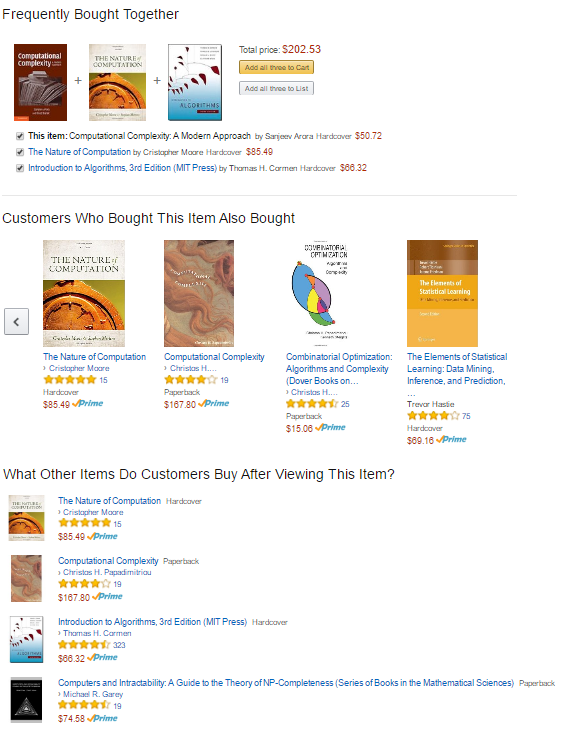
\includegraphics[scale=0.8]{slike/amazon-non_personalized_recom.png}
\caption{Primjeri nepersonaliziranih preporuka na web stranici amazon.com}
\label{fig: amazon nepresonalizirane preporuke}
\end{center}
\end{figure}
\\ Primjeri lista preporuka nepersonaliziranih sustava:
\begin{itemize}[topsep=2pt]
\setlength{\parskip}{0pt}
\item trenutno pregledavane stavke (na vrhu slike \ref{fig: amazon nepresonalizirane preporuke})
\item korisnici koji su kupili neke sadržaje kupili su i sljedeće sadržaje (na sredini slike \ref{fig: amazon nepresonalizirane preporuke})
\item najnoviji sadržaji
\item najprodavaniji sadržaji
\item najpopularniji sadržaji
\item najbolje ocijenjeni sadržaji
\end{itemize}
\bigskip
% odlomak
\par 
Prednost personaliziranih sustava je što analiziraju podatke o korisnicima, njihovim aktivnostima u prošlosti, njihove ocjene proizvoda, njihove odnose s drugim korisnicima, podatke o samom sadržaju i na temelju njih daju personalizirane preporuke za pojedinog korisnika. Kvaliteta sustava mjeri se kroz njegovu sposobnost preporuke sadržaja iz tzv. Long Tail-a. Nepersonalizirani sustavi imaju tendenciju da preporučuju najpopularnije sadržaje, oni postaju sve popularniji i njihov broj se smanjuje. Najpopularniji sadržaji većinom nisu relevanti za pojedinog korisnika. Stoga je važno da sustav daje preporuke ostalih sadržaja kojih je mnogo više, ali koji su relevantni. Slika \ref{fig: long tail} prikazuje odnos tih sadržaja.
% slika
\begin{figure}[!h]
\begin{center}
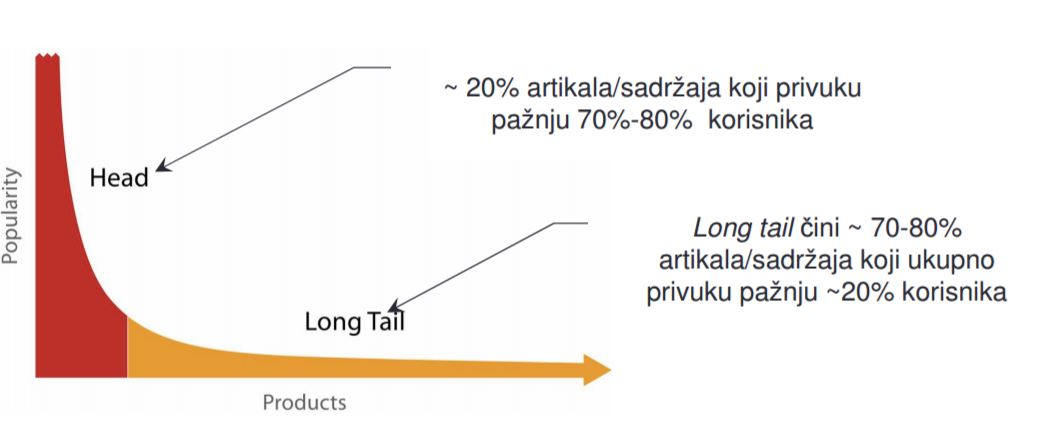
\includegraphics[scale=0.6]{slike/long_tail.jpg}
\caption{Preporučivanje sadržaja (proizvoda i sl.) iz Long Tail-a (J. Jovanović, 2014.)}
\label{fig: long tail}
\end{center}
\end{figure}
% odlomak
\par 
Najčešći nedostaci takvih sustava su: premalo informacija o novom korisniku ili novom sadržaju (eng. cold start), problem skalabilnosti (eng. scalability), problem rapršenosti (eng. sparsity),
korisnik ili sadržaj koji nema sličnosti sa niti jednim drugim korisnikom ili sadržajem (eng. black sheep), problem raznolikosti (eng. diversity) i problem manipulacije sustava (shilling attacks) te pitanje sigurnosti i privatnosti.
% odlomak
\par cold start
% odlomak
\par scalability
% odlomak
\par sparsity
% odlomak
\par black sheep
% odlomak
\par diversity
% odlomak
\par shilling attacks
% odlomak
\par sigurnosti i privatnosti
% odlomak
\par

% lista
\bigskip
\\ Podjela perosnaliziranih sustava:
\begin{itemize}[topsep=2pt]
\setlength{\parskip}{0pt}
\item klasične / tradicionalne metode (eng. classic / traditionals methods)
  \begin{itemize}[topsep=2pt]
  \setlength{\parskip}{0pt}
  \item temeljeni na suradnji (eng. collaborative filtering)
    \begin{itemize}[topsep=2pt]
    \setlength{\parskip}{0pt}
    \item temeljeni na memoriji (eng. memory-based): temeljeni na sličnosti korisnika (eng. user-based ili user-user collaborative filtering), temeljeni na slčnosti objekata (eng. item-based ili item-item collaborative filtering)
    \item temeljeni na modelu (eng. model-based), razvijaju se modeli pomoću algoritama rudarenja podacima (eng. data mining) i strojnog učenja (eng. machine learning)
    \end{itemize}
  \item temeljeni na sadržaju (content-based)
  \item temeljeni na znanju (eng. knowledge-based)
    \begin{itemize}[topsep=2pt]
	\setlength{\parskip}{0pt}
    \item temeljeni na ograničenjima (eng. constraint-based)
	\item temeljeni na slučajevima (eng. case-based)
	\end{itemize}
  \item hibridne metode (eng. hybrid methods)
  \end{itemize}
\item nove metode (eng. novel methods) - web 2.0 (Social Web), web 3.0 (Internet of Things)
    \begin{itemize}[topsep=2pt]
	\setlength{\parskip}{0pt}
    \item temeljeni na osobnosti (eng. personality-based)
    \item temeljeni na demografiji (eng. demographic-based)
    \item temeljeni na zajednicama (eng. social-based ili community-based)
    \item temeljeni na oznakama (eng. tag-based ili keyword-based)
    \item temeljeni na kontekstu (eng. context-based)
	\end{itemize}
\end{itemize}
\bigskip
% poglavlje
\chapter{Sustavi temeljeni na suradnji}
% odlomak
\par Među najpopularnijim algoritmima koji se koriste su oni temeljeni na suradnji. U takvim algoritmima kreiraju se modeli korisnika i pojedinih elemenata sadržaja. Dijelimo ih na one temeljene na sličnosti korisnika, sličnosti korisnika i one temeljene na modelu.
%
\section{Sustavi temeljeni na sličnosti korisnika}
%
Korisnici ocijenjuju objekte na web stranici te se na temelju tih ocjena stvara se model koji pokazuje koliko su slične preferencije korisnica i/ili koliko su slični objekti. Ocjena koju bi korisnik dao nekom objektu, kojeg još nije ocijenio, predviđa se na temelju k najsličnijih korisnika koje zovemo k-najbliži susjedi. Način predviđanja ocjena najčešće je određen sa sljedećom definicijom,
\begin{defn}
Neka je $U$ skup korisnika (eng. users), $I$ skup objekata (eng. items), $u\in U$ neki korisnik te $i\in I$ neki objekt. Korisnici ocijenjuju pojedni objekt što je dano funkcijom $r:U\times I \rightarrow \N$. Ako korisnik njie ocijenio neki objekt tada je vrijednost funkcije r jednaka nuli. $N_i \subseteq U$ je skup od k korinika koji su najsličniji korisniku $u$. Predviđanje koju ocjenu bi dao korisnik $u$ objektu $i$ dana je aritmetičkom sredinom s težinama pri čemu su težine zadane s funkcijom sličnosti korisnika $s:U\times U\rightarrow \R$. 
\[ p:U\times I \rightarrow \R^+, p(u,i) = \overline{r_{u}}+\frac{\sum_{u'\in N_{u,i}}s(u,u')(r(u',i)-\overline{r_{u'}})}{\sum_{u'\in N_{u,i}}|s(u,u')|} \]
Pri čemu je $N_{u,i} \subseteq N_i$ podskup od najbližih korisnika koji su ocijenili objekt i,a $\overline{r_{u'}}$ aritmetička sredina svih ocjena koje je dao korisnik u.
\[ \overline{r_{u}}=\frac{\sum_{i\in I}r(u,i)}{card\{i\in I | r(u,i) \neq 0 \} } \]
\end{defn}
\begin{figure}
\begin{center}
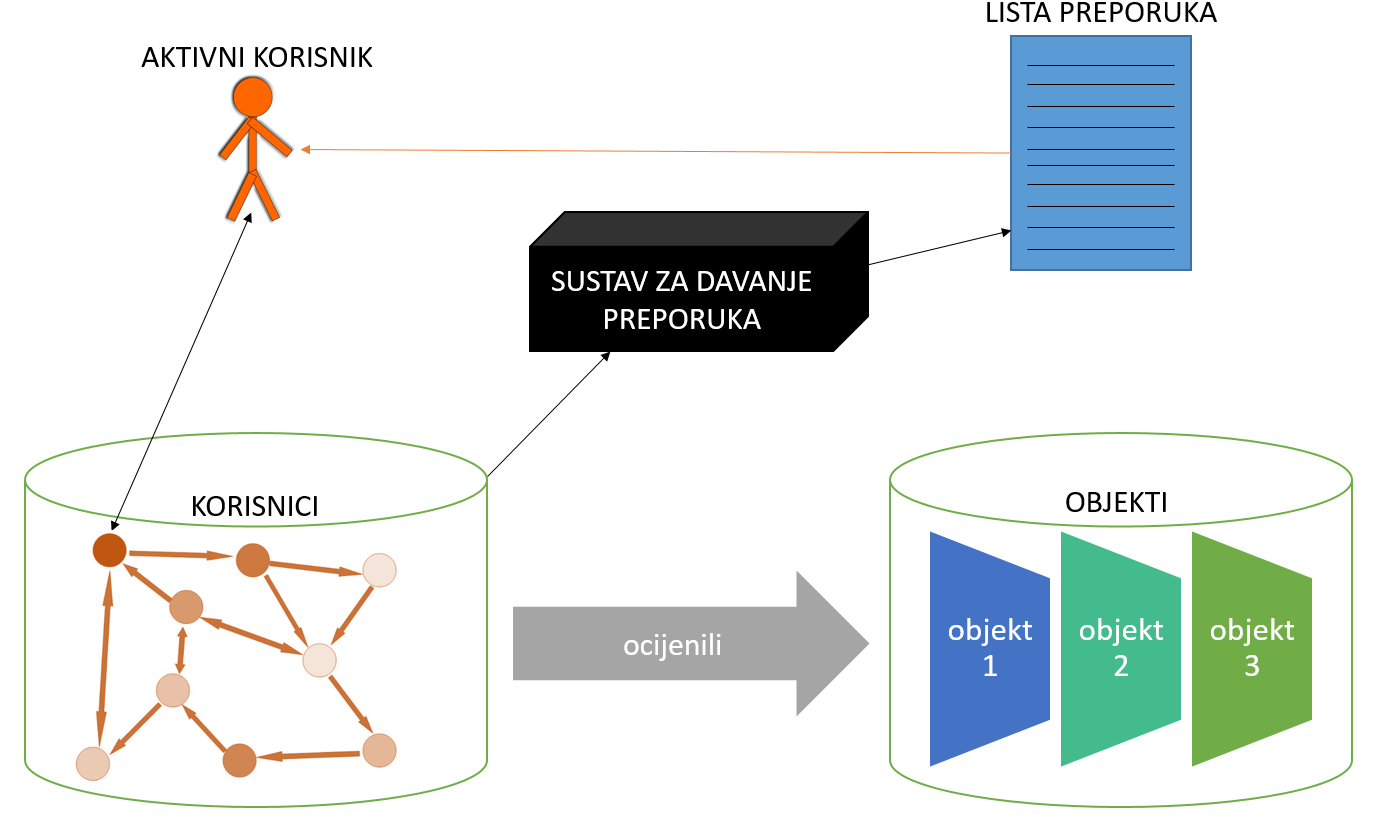
\includegraphics[scale=0.4]{slike/user-based.png}
\caption{Struktura sustava na temelju sličnsti korisnika}
\end{center}
\end{figure}
\bigskip
Za ovaj model moguće je na razne načine zadati funkciju sličnosti između korisnika.
\bigskip
\\Primjeri funkcija sličnosti:
\begin{itemize}[topsep=2pt]
\setlength{\parskip}{0pt}
\item Pearsnov koeficijent korelacije (eng. Pearson correlation)
\item Spearmanov koeficijent korelacije (eng. Spearman rank correlation)
\item kosinusova sličnost (eng. cosine similarity)
\end{itemize}
\begin{defn} (Pearsonov koeficijent korelacije)
\\Neka su $u, v\in U$ neki korisnici i $I_u, I_v$ skup objekata koje je ocijenio korisnik u, odnosno v. Pearsnov koeficijent korelacije zadan je sljedećom formulom.
\[ s:U\times U \rightarrow \R, s(u,v) = \frac{\sum_{i\in I_u\cap I_v}(r(u,i)-\overline{r_u})(r(v,i)-\overline{r_v})}{\sqrt[]{\sum_{i\in I_u\cap I_v}(r(u,i)-\overline{r_u})^2} \sqrt[]{\sum_{i\in I_u\cap I_v}(r(v,i)-\overline{r_v})^2} },  \]
pri čemu je $\overline{r_u}$ aritmetička sredina svih ocjena korisnika u i $\overline{r_v}$ je aritmetička sredina svih ocjena korisnika v.
\end{defn}
%
\begin{rem} (Spearmanov koeficijent korelacije)
\\Računa se kao Pearsonov koeficijent korelacije, samo su ulazne vrijednosti rangovi ocjena, a ne same ocjene. Najvećoj ocjeni dodjeljen je rang 1, sve manjim ocjenama dodijeljeni su sve veći rangovi.
\end{rem}
%
\begin{defn} (kosinusova sličnost)
\\Korisnici su reprezentirani s vektorima $|I|$-dimenzionalnim vektorima pri čemi i-ta pozicja predstavlja ocjenu koju je korisnik dao objektu i. Neka su $r_u$ i $r_v$ vektori koji predstavljaju korinike u i v.
\[ s:U\times U \rightarrow \R, s(u,v) = \frac{r_u\cdot r_v}{||r_u||_2 \: ||r_v||_2} = \frac{\sum_i r(u,i)\: r(v,i) }{\sqrt{\sum_i r(u,i)^2}\:\sqrt{\sum_i r(v,i)^2}}  \]
U prilagođenoj kosinusovoj sličnosti uzima se u obzir i prosječna ocjena korisnika.
\[ s(u,v) = \frac{\sum_i (r(u,i)-\overline{r_u})(r(v,i)-\overline{r_v}) }{\sqrt{\sum_i (r(u,i)-\overline{r_u})^2}\:\sqrt{\sum_i (r(v,i)-\overline{r_v})^2}},  \] 
pri čemu je $\overline{r_u}$ aritmetička sredina svih ocjena korisnika u i $\overline{r_v}$ je aritmetička sredina svih ocjena korisnika v.
\end{defn}
%
\section{Sustavi temeljeni na sličnosti objekata}
\par U ovim sustavima se na temelju ocjena korisnika kreira model u kojem je se određuje sličmost između objekata. Za izračun k-najbliži susjeda u potrebno je $O(|U|)$ koraka, moguće i više, ovisno o načinu računanja funkcije sličnosti. U sustavima sa velikim brojem korisnika potreban je brži način predikcije ocjena. Skalabilnost dobivamo ako prethodno izračunamo susjede svakom objektu, smatra se da su sličnosti između ovjekata stabilniji od sličnosti korisnika, pa kod izračuna predikcija koristimo te unaprijed određene susjede. Objekti su sličniji ako imaju podjednake ocjene korisnika. Slično kao prethodnim sustavima, bira se k-najbližih susjeda nekog objekta i na temelju ocjena korisnika tim susjedima i funkcije sličnosti predviđa se ocjena.
\begin{defn}
Neka je $U$ skup korisnika, $I$ skup objekata, $u\in U$ neki korisnik te $i\in I$ neki objekt. Korisnici ocijenjuju pojedni objekt što je dano funkcijom $r:U\times I \rightarrow \N$. $S \subseteq I$ je skup k-najbližih susjeda objekta $i$. Predviđanje koju ocjenu bi dao korisnik $u$ objektu $i$ dana je aritmetičkom sredinom s težinama pri čemu su težine zadane s funkcijom sličnosti objekata $s:I\times I\rightarrow \R$. 
\[ p:U\times I \rightarrow \R^+, p(u,i) = \frac{\sum_{j\in S}s(i,j)r(u,j)}{\sum_{j\in S}|s(i,j)|} \]
\end{defn}
\begin{rem}
U prethodnoj definicije da se izbjegnu predikcije koje mohu biti negativne trebaju se onda uzeti u obzir samo objekti koji imaju nenegativnu sličnost. U sustavima koje je moguće dati samo binarnu ocjenu (0 ili 1) potrebno je drugačije definirati predikciju, može se definirati samo kao suma sličnosti.
\end{rem}
Također i u ovom modelu potrebno je odrediti funkciju sličnosti. Kosinusova sličnost i Pearsonov koeficijent se definira analogno kao u prethodno definiranim sustavim pri čemu se u praksi pokazuje da je puno bolja kosinusova sličnost.
\bigskip
\\Primjeri funkcija sličnosti:
\begin{itemize}[topsep=2pt]
\setlength{\parskip}{0pt}
\item kosinusova sličnost i prilagođena kosinusova sličnost
\item Pearsnov koeficijent korelacije 
\item Spearmanov koeficijent korelacije 
\item uvjetna vjerorajtnost (eng. conditional probability) - koristi se u sustavi s binarnom ocjenom
\end{itemize}
\begin{figure}
\begin{center}
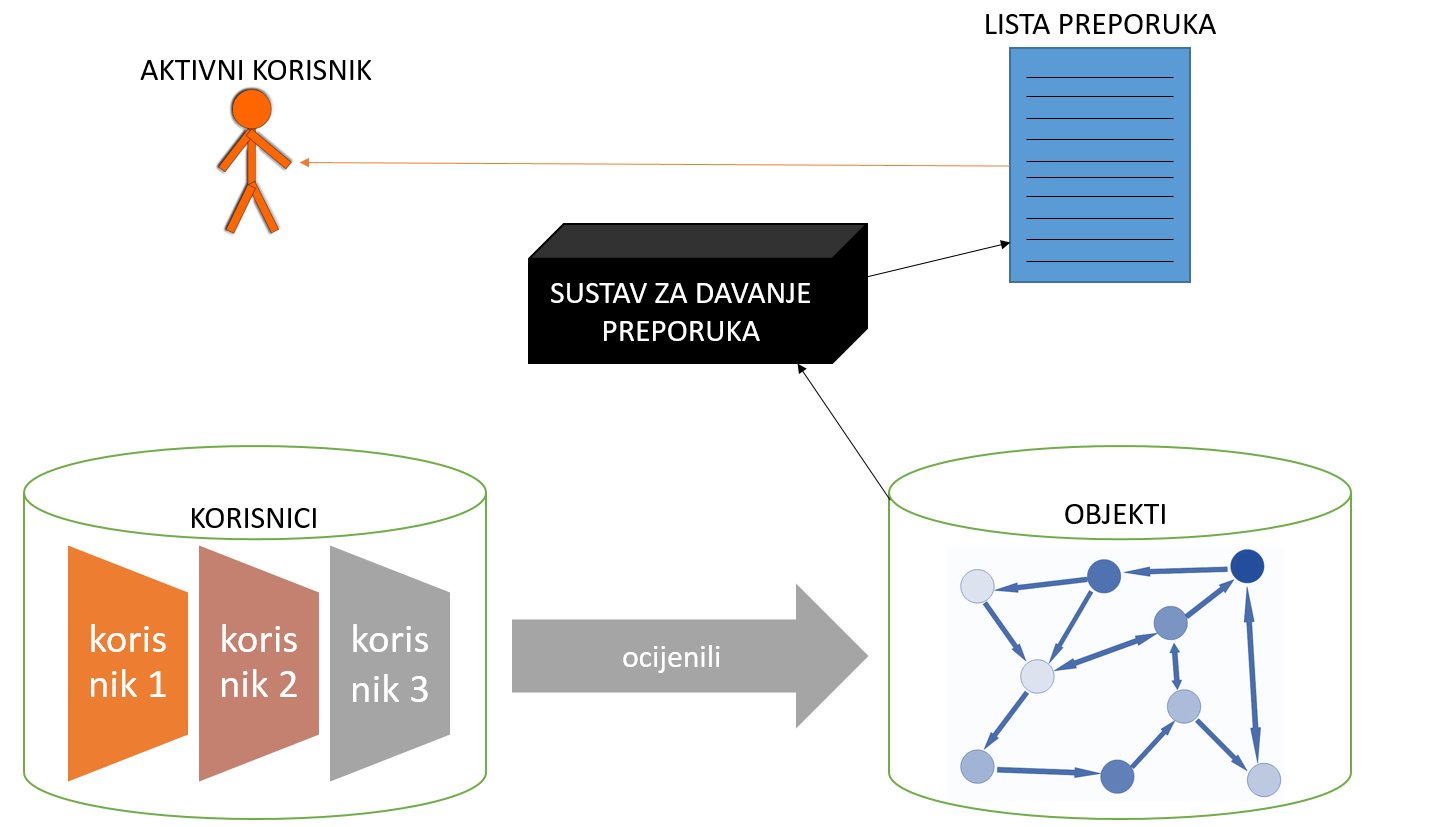
\includegraphics[scale=0.4]{slike/item-based.png}
\caption{Struktura sustava na temelju sličnsti objekata}
\end{center}
\end{figure}
%
\section{Sustavi temeljeni na modelu}
%
Prethodno dva opisana sustava temnelje svoje predikciju na svim ocjenama korisnika, tj. na cijeloj bazi korisnika i objekata pa takve sustave zovemo temeljeni na memoriji. Sustavi temeljeni na modelu kreiraju neki model pomoću algoritama rudarenja podataka  i strojnog učenja (eng. machine learning) nad podacima. Prednost ovakvog pristupa je što se postižu bolja skalabilnost (brže vrijeme izvršavanja i manje memorije kod većih sustava) i postižu se bolje predikcije na rasprešenim podacima. Nedostatatak je taj što je potrebna zahtjevna izrada modela i treba paziti koji se model primjenuje jer dolazi do određenog gubitka podataka.
\bigskip
\\ Neki od algoritama za izradu modela:
\begin{itemize}
\item SVD redukcija dimenzionalnosti (eng. SVD-based reduction dimensionality)
\item analiza glavnih componenti (eng. principle component analysis)
\item asocijacijska pravila
\item klasifikatori: stabla odluke
\item 	Baysove mreže
\item 	neuronske mreže
\item 	SVM
\item grupiranje podataka
\end{itemize}
%
\subsection{SVD redukcija dimenzionalnosti}
\par
Vektori u sustavima temeljeni na memoriju koji predstavljaju korisnika su dimenzija $|I|$, ondnosmo ono koji predstavjaju objekta su dimenzija $|U|$. Kako sustav ima puno korisnika i objekta vektori su velikih dimenzija. Redukcijom dimenzija dobivamo bolje performanse i riješavamo se šuma. Definiramo singularnu dekompoziciju matrice i kako se primjenjuje u preporukama.
\begin{defn} (Dekompozicija singularnih vrijednosti, eng. singular value decomposition, SVD)
\\Neka je M realna matrica, $M\in \R^{m\times n}$. M se može zapisati kao $M=U\Sigma V^*$, pri čemu je U $m\times m$ ortogonalna matrica, a V* $n\times n$ ortogonalna matrica. Matrica $\Sigma$ je $m\times n$ dijagonalna matrica pri čemu su dijagonalni elementi $\sigma_i$ poredani od najvećeg prema najmanjem i zovemo ih singularnim vrijednostima matrice M. Matrica ranga k ima k singularnih vrijednosti, pa je $\sigma_i=0$ za $i>k$.
\\ Stupci matrice U zovemo lijevi singlurani vektori matrice M, a stupce matrice V desni singularni vektori matrice M.
\\ Lijevi singularni vektori jednaki su otronormiranim svojstvenim vektorima matrice MM*, desni singularni vektori jednaki su otronormiranim svojstvenim vektorima matrice M*M, a nenegativne singularne vrijednosti su korjeni nenagativnih svojstvenih vrijednosti matrica MM* (jednake i za M*M).
\\ Kako je M realna matrica tada $V^*=V^T$ i V je ortogonalna tj. $VV^T=1$.
\end{defn}
Neka su u daljnjem tekstu $m:=|U|$ i $n:=|I|$. Prostore s m i n dimenzijama želimo reducirati na prostor dimenzije k, taj prostor ćemo zvati prostor značajki. SVD dekompozicijom otkrivamo k značajki i preferenciju korisniku prikažemo u prostoru značajki te preporučujemo najbliže vektore objekta prikazanih u tom prostoru.
\begin{defn} Neka je R matrica ocjena dimenzija $m\times n$, $r_{i,j}:=r(i,j)$. Matrica ocjena R se može aproksimirati dekompozicijom singularnih vrijednosti $R \approx \hat{U} \hat{\Sigma} \hat{I}^T$. $\Sigma$ je matrica dimenzija $\hat{k}\times \hat{k}$ koja sadrži $\hat{k}$ najveće singularne vrijednosti matrice R, $\hat{k}<k=rang(R)$. Time dobovima preslikavanje vektora korinika i objekta u prostor značajki dimenzije k. Neke je $\hat{u}_l$ l-ti redak matrice $\hat{U}$, $\sigma_l$ l-ti dijagonalni element matrice $\hat{\Sigma}$ i $\hat{i}_l$ l-ti stupac matrice $\hat{I}^T$. Predikcija je dana s:
\[ p:U\times I \rightarrow \R^+, p(u,i) = \sum_{l=1}^k \hat{u}_l \sigma_l \hat{i}_l \]
\end{defn}
\begin{rem} 
Koristeći Frobeniusovu normu kao mjeru greške tada je singularna dekompozicija matrice R najbolja aproksimacija s matricom ranga $\hat{k}$.
\end{rem}
\begin{defn} $\tilde{R}$ je normalizirana matrica matrice R pri čemu je $\tilde{r}_{u,i} = (r_{u,i}-\mu_i)/\sigma_i$. $\mu_i$ je aritmetička sredina ocjena objekta i, a $\sigma_i$ je njihova varijanca.
\end{defn}
\begin{figure}
\begin{center}
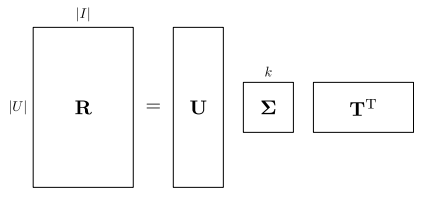
\includegraphics[scale=0.8]{slike/svd_decom.png}
\caption{Singularna dekompozicija matrice R}
\end{center}
\end{figure}
%
\subsection{Analiza glavnih komponenti}
Opis!
\begin{defn} (Svojstveni vektor i svojstvena vrijednost)
\\Netrivijalni vektor x dimenzije n ($x\in \R^n$ i $x\neq 0$) zovemo svojstveni vektor realne kvadratne matrice A, $A\in \R^{n\times n}$, ako vrijedi $Ax=\lambda x$ za neki skalar $\lambda \neq 0$. Skalara $\lambda$ ako postoji onda je jedinstven i zovemo ga svojstvena vrijednost matrice A pridružena svojstvenom vektoru x. 
\end{defn}
\begin{defn} (Dekompozicija svojstvenih vrijednosti ili spektralna dekompozicija, eng. eigenvalue decomposition ili spectral decomposition, EDV)
\\Neka je A realna kvadratna matrica, $A\in \R^{n\times n}$, koja ima n linearno nezavisnih svojstvenih vektora $q_i,  i = 1,2,3,...,n.$ Tada se matrica A može zapisati kao $A=Q\Lambda Q^{-1}$, pri čemu je Q matrica sa stupcima koji su jednaki svojstvenim vrijednostima, a $\Lambda$ je dijagonalna matrica gdje je i-ti dijagonalni element jednak svojstvenoj vrijednosti $\lambda_i$ matrice A pridružena svojstvenom vektoru $q_i$.
\\ Ako je A simetrična kvadratna matrica tada se A može zapisati kao $A=Q\Lambda Q^{T}$, gdje je Q ortogonalna matrica.
\end{defn}
\begin{defn}
Neka je $C=\frac{1}{|U|-1}\tilde{R}^T\tilde{R}$ matrica kovarijanci. Matrica C je realna simetrična pozitvno semidefinitna matrica, pa postoji njena spektralna dekompozicija. Analiza glavnih komponenti aproksimira matricu $\tilde{R}$ sa spektralnom dekompozicijom matrice s njenih $\hat{k}$ najvećih svojstvenih vrijednosti, $\tilde{R}\approx \hat{Q}\hat{\Sigma}\hat{Q}^T$. Predikcija je dana s:
\[ p:U\times I \rightarrow \R^+, p(u,i) = ? \]
\end{defn}
%
\subsection{Stabla odluke}
%
\subsection{Baysove mreže}
%
\subsection{Neuronske mreže}
%
\subsection{Markovljevi procesi}
%
\subsection{Grupiranje podataka}
%
\chapter{Sustavi temeljeni na sadržaju}	

%
\chapter{Sustavi temeljeni na znanju}	
%
\chapter{Pregled novih metoda}	
%
\chapter{Sustav temeljen na oznakama}	
%
\chapter{Evaluacija sustava}	
%
\chapter{Trenutni izazovi i budućnost}	
%
\chapter{Primjeri pisanja algoritama}	
\begin{algorithm}[H]
\KwIn{
Integers $a \geq 0$ and $b\geq 0$}
\KwOut{\textsc{GCD} of $a$ and $b$}
\While{$b \neq 0$} {
$r \leftarrow a \bmod b$\;
$a \leftarrow b$\;
$b \leftarrow r$\;
}
\caption{Euclidean algorithm}
\end{algorithm}

\begin{lstlisting}[caption=Test]
function [ P ] = kNN_user_based_prediction( R, k, similarity_measure ) 
    m = size(R,1);
    n = size(R,2);
    mean_userRates = sum(R, 2)./sum(R~=0, 2);
    S = similarity_measure( R );
    [~, N] = sort(S,2,'descend');
    N = N(:,1:k);
    P = zeros(m,n);
    for u = 1:m
        for i = 1:n
            if R(u,i) == 0
                P(u,i) = mean_userRates(u) + ...
                dot( (R(N(u,:),i)~=0)' .* S(u,N(u,:)), R(N(u,:),i) - ...
                mean_userRates(N(u,:)) ) / norm( (R(N(u,:),i)~=0)' .* S(u,N(u,:)), 1 );
            else
                P(u,i) = R(u,i);
            end
        end
    end
end
\end{lstlisting}

\lstinputlisting[breaklines=true, caption=Test from file]{kodovi/kNN_user_based_recom.m}

% Na kraju diplomkog rada stavlja se  bibliografija
% Najprije definiramo nacin prikazivanja bibliografije, u ovom slucaju verzija amsplain stila
\bibliographystyle{babamspl} % babamspl ili babplain

% U datoteku diplomski.bib se stavljaju bibliografske reference
% Bibliografske reference u bib formatu se mogu dobiti iz MathSciNet baze, Google Scholara, ArXiva, ...
\begingroup
\raggedright
\bibliography{bibliografija/diplomski}
\nocite{*}
\endgroup



\pagestyle{empty} % ne zelimo brojanje sljedecih stranica

% I na koncu idu sazeci na hrvatskom i engleskom

\begin{sazetak}
Ukratko ...
\end{sazetak}

\begin{summary}
In this ...
\end{summary}

% zivotopis
\begin{cv}
Rođen sam 18. kolovoza 1991. godine u Puli. U Rovinju sam završio Osnovnu školu Jurja Dobrila. Već u osnovnoj školi pokazujem interes za matematiku i informatiku posebice za programiranjem te sam sudjelovao na brojnim županijskim i državnim natjecanjima. Bio sam član Udruge tehničke kulture "Galileo Galilei" u Rovinju, a kasnije za udrugu vodim radionicu "Izrada web stranica" za osnovnoškolce. Uspješnim polaganjem državne mature 2010. godine završio sam prirodoslovno-matematičku gimnaziju u Srednjoj školi Zvane Črnje u Rovinju. Iste godine upisujem sveučilišni preddiplomski studij Matematike na Prirodoslovno-matematičkom fakultetu u Zagrebu, zatim 2015. godine  upisujem sveučilišni diplomski studij Računarstva i matematike. Tijekom studija radio sam kao nastavnik matematike i računarstva u Srednjoj školi Zvane Črnje u Rovinju i u Srednjoj strukovnoj školi u Samoboru te sam bio demonstrator iz kolegija Građa računala. Za fakultet redovito sam sudjelovao u sportskim natjecanjima iz dvoranske odbojke i odbojke na pijesku. 
\end{cv}

\end{document}